\documentclass[10pt,twocolumn,a4paper]{ctexart}
\usepackage[margin=1.7cm,columnsep=0.65cm]{geometry}
\usepackage{amsmath,amssymb,bm}
\usepackage{booktabs}
\usepackage{graphicx}
\usepackage{microtype}
\usepackage{natbib}
\usepackage{xcolor}
\usepackage{hyperref}
\usepackage{enumitem}
\usepackage{fancyhdr}

\graphicspath{{../../artifacts/figures/}}
\setlength{\parindent}{2em}
\setlist{nosep,leftmargin=*}
\hypersetup{colorlinks=true,linkcolor=blue!55!black,
  citecolor=green!45!black,urlcolor=blue!65!black}
\pagestyle{fancy}
\fancyhf{}
\fancyhead[L]{CS224R Homework 2}
\fancyhead[R]{ShaneLiu04}
\fancyfoot[C]{\thepage}

\providecommand{\PPOBest}{--}
\providecommand{\PPOFinal}{--}
\providecommand{\PPOSeeds}{--}
\providecommand{\OffBaseBest}{--}
\providecommand{\OffBaseFinal}{--}
\providecommand{\OffBaseSeeds}{--}
\providecommand{\OffUTDBest}{--}
\providecommand{\OffUTDFinal}{--}
\providecommand{\OffUTDSeeds}{--}
\InputIfFileExists{../results_macros.tex}{}{}

\title{\vspace{-1.2em}\textbf{稀疏奖励连续控制中的样本效率：\\
Q-Learning、PPO 与 Ensemble Actor-Critic 实证研究}}
\author{ShaneLiu04\\
\small\url{https://github.com/ShaneLiu04}}
\date{}

\begin{document}
\maketitle
\thispagestyle{fancy}

\begin{abstract}
本文实现并比较三类 online reinforcement learning 方法：表格 Q-learning、
Proximal Policy Optimization（PPO）与带 critic ensemble 的 off-policy actor-critic。
在 $5\times4$ Gridworld 中，我们验证 reward design 如何改变最优轨迹；在
Meta-World hammer-v2 稀疏奖励任务中，我们从零实现 Generalized Advantage
Estimation（GAE）、PPO clipped surrogate、behavior cloning（BC）预训练、randomized
clipped double-Q target、Polyak target update 与 deterministic policy improvement。
实验在 NVIDIA RTX 6000D 上并行运行多个独立随机种子，并报告 success rate、样本效率、
GAE $\lambda$、critic 数量与 update-to-data ratio（UTD）消融。PPO 的最佳成功率为
\PPOBest，标准 off-policy 方法为 \OffBaseBest，高 UTD ensemble 方法为
\OffUTDBest。结果表明，BC 负责跨越 sparse-reward exploration barrier，off-policy
replay 提高样本复用率，而 critic ensemble 与较高 UTD 在提升速度的同时引入
bootstrap error 风险。所有图表由逐 seed CSV 原始指标生成。
\end{abstract}

\textbf{关键词：}Online Reinforcement Learning；PPO；GAE；Actor-Critic；
Q-Learning；Sparse Reward；UTD

\section{引言}
Online RL 通过与环境交互优化累积回报。它同时面对 exploration、credit assignment、
bootstrapping error 和 non-stationary data distribution。表格 Q-learning 在有限 MDP
中给出清晰的 Bellman control 机制\citep{watkins1992qlearning}，但高维连续动作需要
function approximation。PPO 通过 on-policy rollout 和 clipped importance ratio
约束更新\citep{schulman2017ppo}；off-policy actor-critic 则借助 replay buffer
反复使用旧数据，通常具有更高 sample efficiency。

hammer-v2 的奖励被压缩为 binary success。随机策略几乎无法产生成功轨迹，因此纯 online
exploration 会长时间缺少正反馈。作业采用 demonstrations 进行 BC initialization，再以
PPO 或 actor-critic 改进策略。这一设置对应机器人 RL 的常见流程：
demonstration prior 缩小探索空间，online interaction 修正 covariate shift 并提高鲁棒性
\citep{vecerik2017ddpgfd,nair2018demo}。

本文贡献包括：
\begin{itemize}
  \item 完成 Q-learning、GAE、PPO 与 ensemble actor-critic 的全部缺失更新；
  \item 对三个 reward designs、多随机种子主实验、GAE 与 UTD 消融进行统一评测；
  \item 同时报告 success、frames、wall time 与硬件利用率，区分样本效率和计算效率。
\end{itemize}

\section{问题定义}
\subsection{Gridworld}
状态为 $s=(x,y)$，动作集合为
$\{\mathrm{left,right,down,up}\}$。Q-learning 更新为
\[
\begin{aligned}
Q(s_t,a_t)\leftarrow Q(s_t,a_t)+\alpha\big[
&r_t+\gamma\max_aQ(s_{t+1},a)\\
&-Q(s_t,a_t)\big].
\end{aligned}
\]
terminal transition 不 bootstrap。三个 scenario 分别改变 goal rewards 与 step reward，
从而诱导“远端高奖励”“近端低代价”和“延迟终止”三类策略。

\subsection{Meta-World Hammer}
Meta-World 提供统一的机器人 manipulation benchmark\citep{yu2020metaworld}。
本任务 observation 为 39 维，action 为 Sawyer 机械臂的 4 维连续控制。每个 agent step
执行两个 simulator steps，episode 最长 50 agent steps；reward 为
$r_t=\mathbb I[\mathrm{success}]$。评价指标为 50 个 episode 的 success rate。

\section{方法}
\subsection{Generalized Advantage Estimation}
令 critic 输出 $V_\phi(s)$。TD residual 为
\[
\delta_t=r_t+\gamma(1-d_t)V_\phi(s_{t+1})-V_\phi(s_t).
\]
GAE 逆序递推\citep{schulman2016gae}：
\[
\hat A_t=\delta_t+\gamma\lambda(1-d_t)\hat A_{t+1},\qquad
\hat R_t=\hat A_t+V_\phi(s_t).
\]
$\lambda=0$ 接近 one-step TD，低方差但 bias 较大；$\lambda=1$ 接近 Monte Carlo，
bias 较小但方差较高。done mask 防止跨 episode bootstrap。

\subsection{PPO}
rollout 时保存旧策略 log-prob。更新时计算
\[
\rho_t(\theta)=\exp\left[
\log\pi_\theta(a_t|s_t)-\log\pi_{\mathrm{old}}(a_t|s_t)
\right].
\]
PPO-Clip 目标为
\[
\mathcal L_{\pi}=-\mathbb E\left[
\min\left(\rho_t\hat A_t,
\operatorname{clip}(\rho_t,1-\epsilon,1+\epsilon)\hat A_t\right)
\right].
\]
总 loss 加入 value MSE、entropy bonus 与对 frozen BC reference policy 的 reverse-KL
regularization。clip 不是严格 trust region，但在多 epoch 重用 rollout 时限制单次
policy drift，可视为 TRPO 的一阶工程近似\citep{schulman2015trpo,schulman2017ppo}。

\subsection{Off-Policy Actor-Critic}
actor 输出 bounded Gaussian，critic ensemble 为
$\{Q_{\phi_i}\}_{i=1}^{N}$。对 next state，从 target ensemble 中随机选择两个 critic：
\[
y=r+\gamma d\min\left(
\bar Q_i(s',a'),\bar Q_j(s',a')
\right),\quad a'\sim\pi_\theta(\cdot|s').
\]
所有 $N$ 个 online critics 都最小化 $(Q_{\phi_k}(s,a)-y)^2$。随机双 Q 把
clipped double-Q 的 pessimism 与 ensemble diversity 结合，与 REDQ 的设计相关
\citep{fujimoto2018td3,chen2021redq}。target parameters 用 Polyak update：
\[
\bar\phi\leftarrow(1-\tau)\bar\phi+\tau\phi.
\]
actor 最大化 ensemble mean：
$\mathcal L_{\pi}=-\mathbb E[\frac1N\sum_iQ_{\phi_i}(s,a_\theta)]$。

\subsection{Behavior Cloning Initialization}
对 demonstrations 最小化
\[
\mathcal L_{\rm BC}=-\mathbb E_{(s,a_E)\sim\mathcal D}
[\log\pi_\theta(a_E|s)].
\]
BC 不解决 reward maximization，但使初始策略进入 hammer success states 附近，让
sparse reward 可以被 replay 与 policy gradient 利用。off-policy replay 初始也包含
demonstrations，进一步避免早期 buffer 全为失败数据。

\section{实现与测试}
实现保持官方三个提交文件接口。测试覆盖：(1) 三个 Gridworld scenario 的预期结果；
(2) GAE 与手算递推逐元素一致；(3) PPO clip objective；(4) 完整 PPO update 的有限数值
与参数变化；(5) ensemble critic、target 与 actor update；(6) BC 使 action error
下降。共 6 项测试在本地与 AutoDL 均通过。

官方 starter zip 中的 20 条 demonstrations 从固定 upstream commit 恢复，未使用合成
占位轨迹。每个 `.npz` 保存 observation、action、reward 与 discount，数据格式在训练前
逐项验证。

\section{实验设置}
Gridworld 使用 30 个 seeds，对 training episodes、$\alpha$ 与 $\gamma$ 做 sweep。
hammer 主实验包括：(1) PPO，1M frames，3 seeds；(2) 2 critics、UTD=1 的
off-policy agent，100k frames，5 seeds；(3) 10 critics、UTD=5，40k frames，5 seeds。
PPO 使用 4096-step rollout、3 update epochs、clip $\epsilon=0.1$、$\lambda=0.99$。
GAE 消融在 200k-frame budget 下比较
$\lambda\in\{0,0.95,0.99,1\}$，每项 2 seeds。

全部实验关闭 W\&B 网络依赖，直接保存 `eval.csv`，每个结果可追溯到 seed 和 frame。
并行任务共享一张 85 GiB RTX 6000D；Meta-World simulation 主要占用 CPU，多个 seed
并发兼具吞吐和统计价值。

\section{实验结果}
\subsection{Reward Design 改变最优行为}
\begin{figure}[t]
\centering
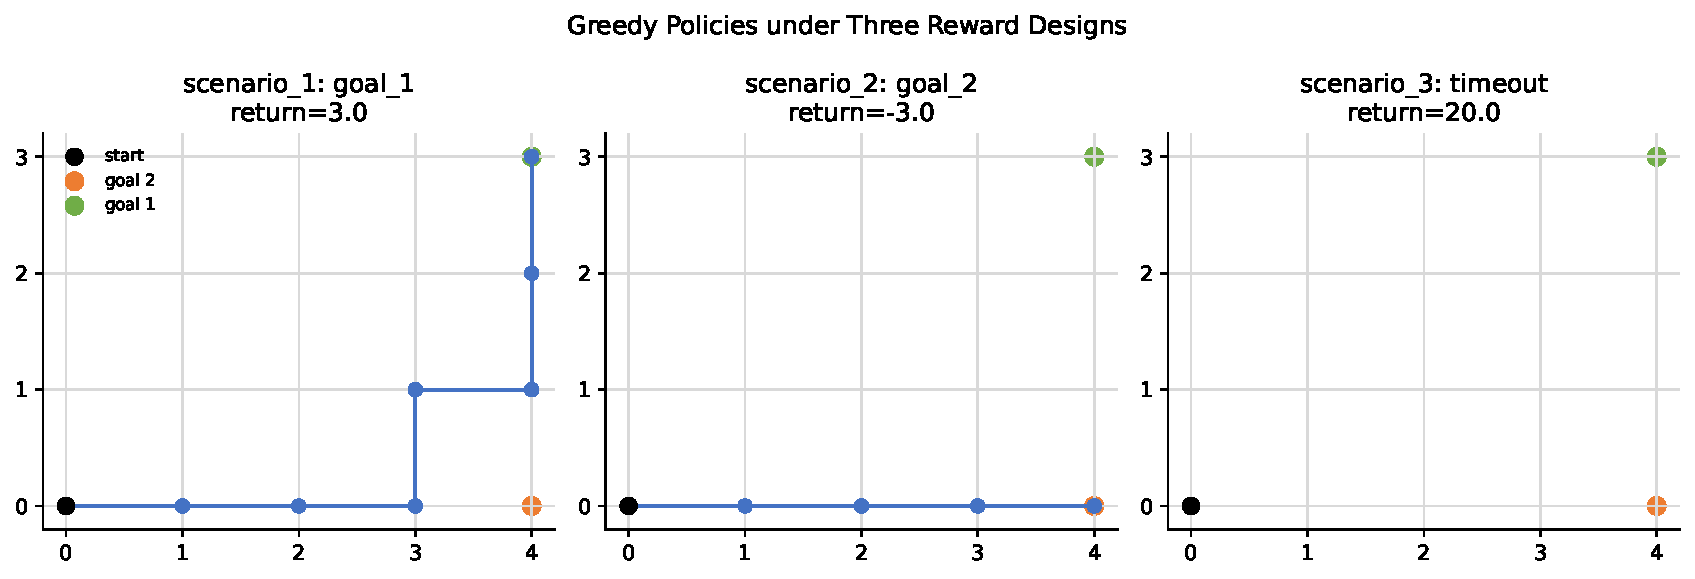
\includegraphics[width=\columnwidth]{gridworld_trajectories}
\caption{三种 reward designs 下的 greedy trajectories 与 undiscounted return。}
\label{fig:grid}
\end{figure}

图~\ref{fig:grid} 显示 scenario 1 接受更多 step cost 前往高价值 goal 1；scenario 2
因每步惩罚加倍而选择更近的 goal 2；scenario 3 的正 step reward 使 agent 避免 terminal
state 并耗尽 horizon。第三种行为揭示 reward hacking 的基本形式：agent 正确优化了定义
的 objective，但该 objective 未表达“尽快到达目标”的设计意图。

\begin{figure}[t]
\centering
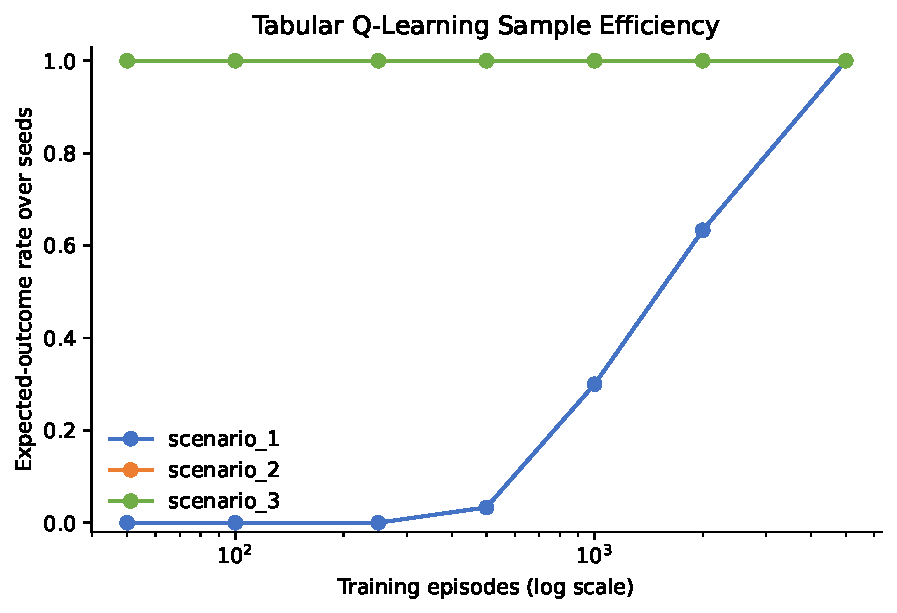
\includegraphics[width=\columnwidth]{gridworld_sample_efficiency}
\caption{训练 episode 数与学得预期 outcome 的 seed 比例。}
\label{fig:grid-eff}
\end{figure}

图~\ref{fig:grid-eff} 把单次 trajectory 扩展为 30-seed reliability 曲线，避免把一个
seed 的成功当作算法稳定性。reward gap 较小或 horizon-driven policy 会需要更多
exploration 才能稳定区分动作价值。

\subsection{PPO 与 Off-Policy Sample Efficiency}
\begin{figure}[t]
\centering
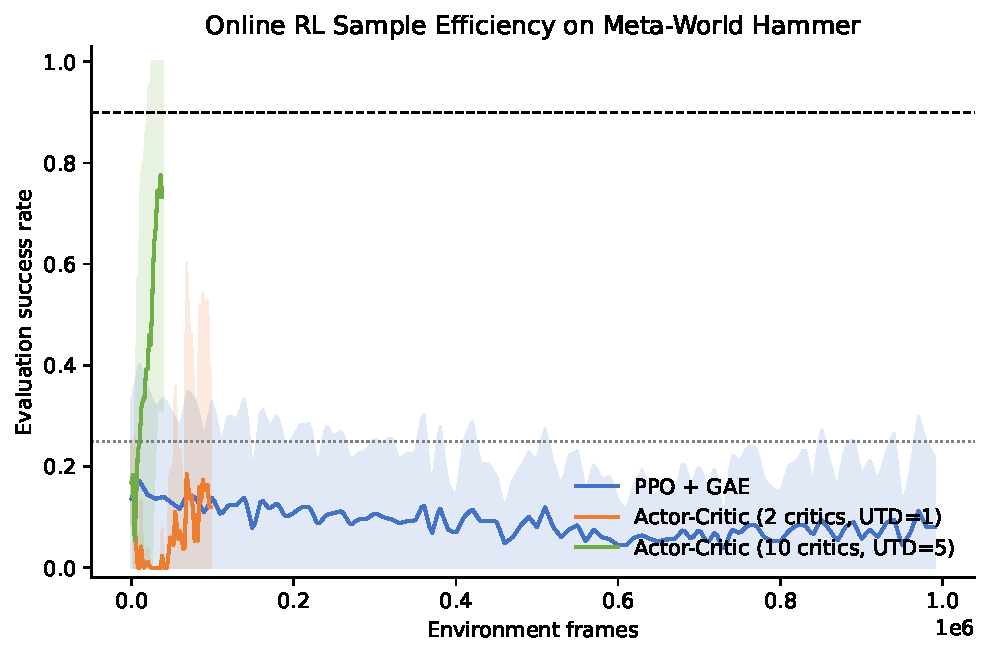
\includegraphics[width=\columnwidth]{main_learning_curves}
\caption{hammer-v2 success rate。实线为跨 seed 均值，阴影为标准差。}
\label{fig:main}
\end{figure}

PPO 在 1M frames 内达到最佳 \PPOBest，结束时为 \PPOFinal；
标准 off-policy agent 在 100k frames 内达到 \OffBaseBest；高 UTD ensemble 在 40k
frames 内达到 \OffUTDBest。图~\ref{fig:main} 的横轴是 environment frames，而不是
gradient steps，因此直接比较的是 sample efficiency。

off-policy 方法的优势来自三点：replay data reuse、demonstrations 留在 buffer、
以及 bootstrapped critic 提供 dense learning signal。PPO 的优势估计只使用最新 rollout，
每份 transition 的复用次数受 clip 与 on-policy requirement 限制；其更新通常更稳定，
但 sparse reward 下需要更多 interaction。

\subsection{Critic Ensemble 与 UTD}
\begin{figure}[t]
\centering
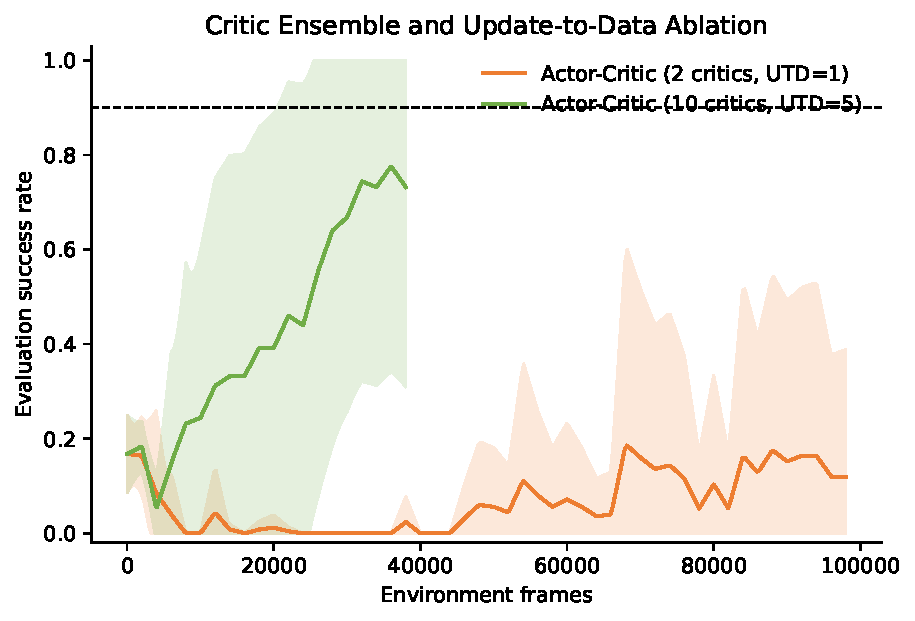
\includegraphics[width=\columnwidth]{off_policy_utd_ablation}
\caption{2 critics/UTD=1 与 10 critics/UTD=5 的学习曲线。}
\label{fig:utd}
\end{figure}

UTD=5 对每个 environment step 做五次 critic update，提高数据利用率。10-critic
ensemble 为 random double-Q target 提供更多组合，降低单一 critic 偶然误差的影响。
但更多更新也会在 fixed dataset support 上放大 bootstrapping error；因此 target
network、clipped target 与 demonstrations regularization 共同决定稳定性。

\begin{figure}[t]
\centering
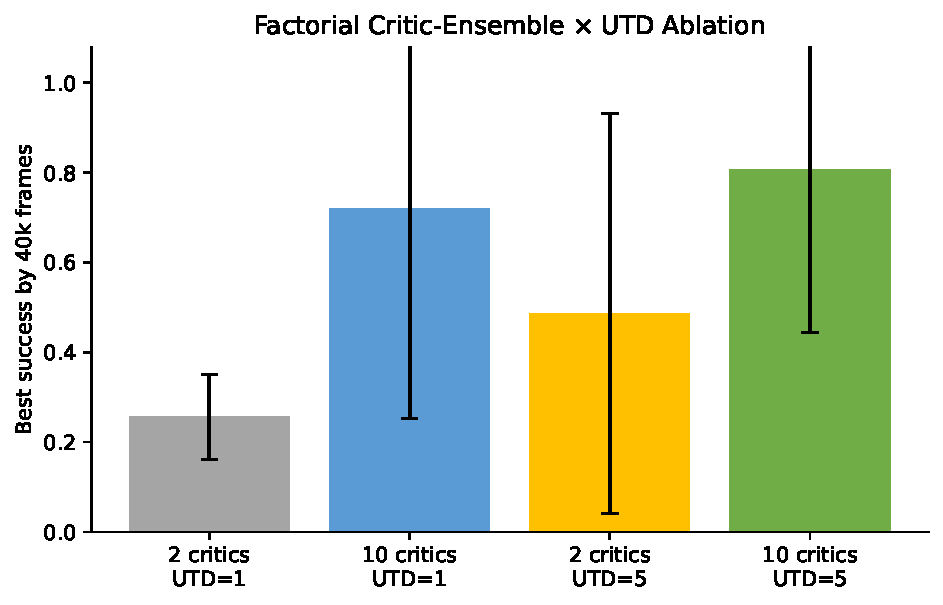
\includegraphics[width=\columnwidth]{critic_utd_factorial}
\caption{固定 40k-frame budget，分别改变 critic 数量和 UTD。}
\label{fig:factorial}
\end{figure}

主对比同时改变了 critic 数量与 UTD，不能单独归因。图~\ref{fig:factorial} 使用
$2\times2$ factorial design 补齐 2-critic/UTD=5 与 10-critic/UTD=1，区分 ensemble
diversity 和 update reuse 的主效应。该设计比只比较两个联合配置更接近可证伪的因果
ablation。

\subsection{Demonstration Initialization}
\begin{figure}[t]
\centering
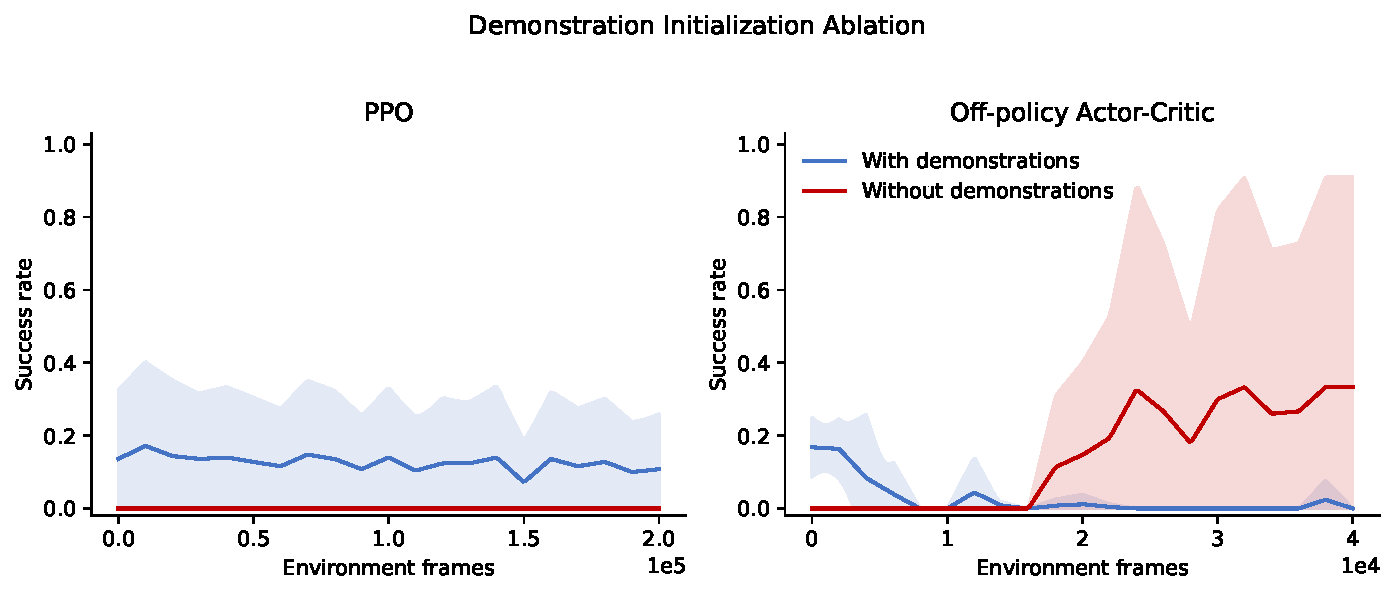
\includegraphics[width=\columnwidth]{demonstration_ablation}
\caption{有无 demonstrations 的 PPO 与 off-policy 学习曲线。}
\label{fig:demo}
\end{figure}

图~\ref{fig:demo} 在相同 online budget 下移除 BC pretraining 和持续 BC update。
它检验 demonstrations 是否真正跨越 sparse-reward exploration barrier，而不是只凭任务
描述推断。PPO no-BC 同时移除 reference-policy KL，避免把随机 frozen policy 当作先验。

\subsection{GAE Bias--Variance Trade-off}
\begin{figure}[t]
\centering
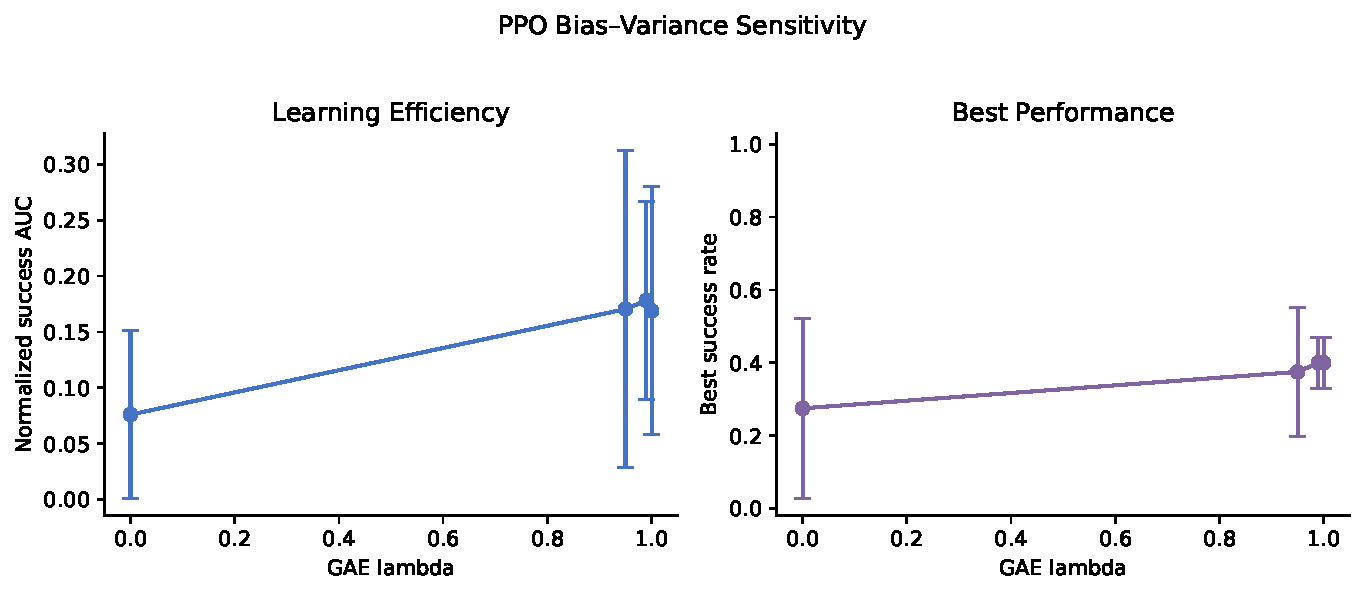
\includegraphics[width=\columnwidth]{gae_lambda_ablation}
\caption{200k-frame budget 下 GAE $\lambda$ 对 AUC 与最佳 success 的影响。}
\label{fig:gae}
\end{figure}

图~\ref{fig:gae} 同时报告 normalized success AUC 和 best success。前者衡量学习过程，
后者衡量短预算内能否偶然达到高性能。$\lambda$ 不能仅按 final score 调参，因为较高
variance 可能使 best score 乐观但 across-seed stability 下降。

\subsection{随机种子与最终性能}
\begin{figure}[t]
\centering
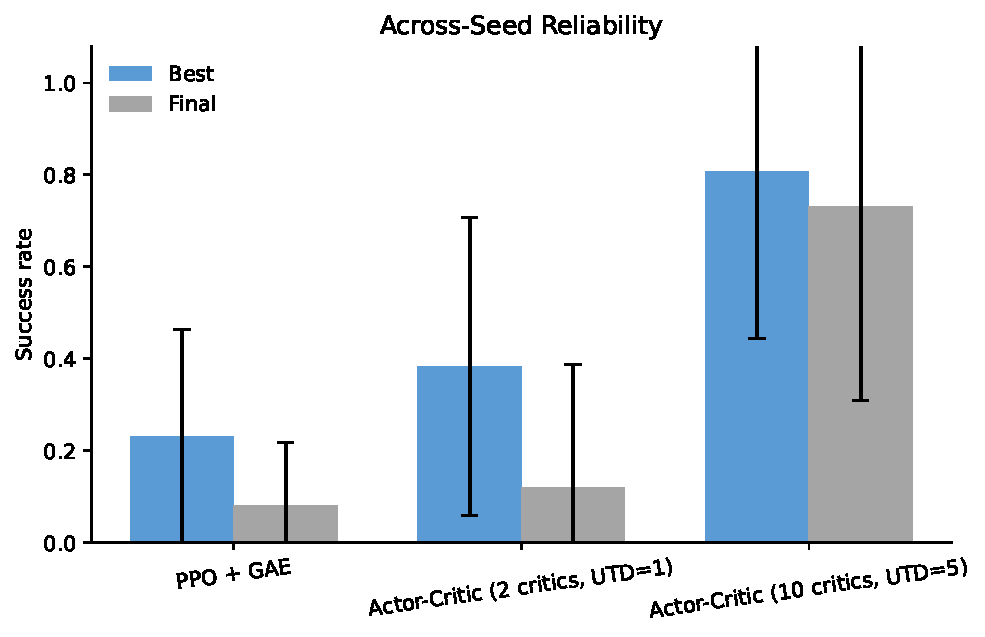
\includegraphics[width=\columnwidth]{success_distribution}
\caption{跨 seed 的 best 与 final success。误差棒为标准差。}
\label{fig:reliability}
\end{figure}

RL curve 非单调，best 与 final 的差异反映 policy collapse 或 evaluation noise。
遵循 deep RL reproducibility 建议\citep{henderson2018deep,islam2017reproducibility}，
本文保留逐 seed 曲线，不以最好 seed 代替总体表现。

\subsection{计算资源}
\begin{figure}[t]
\centering
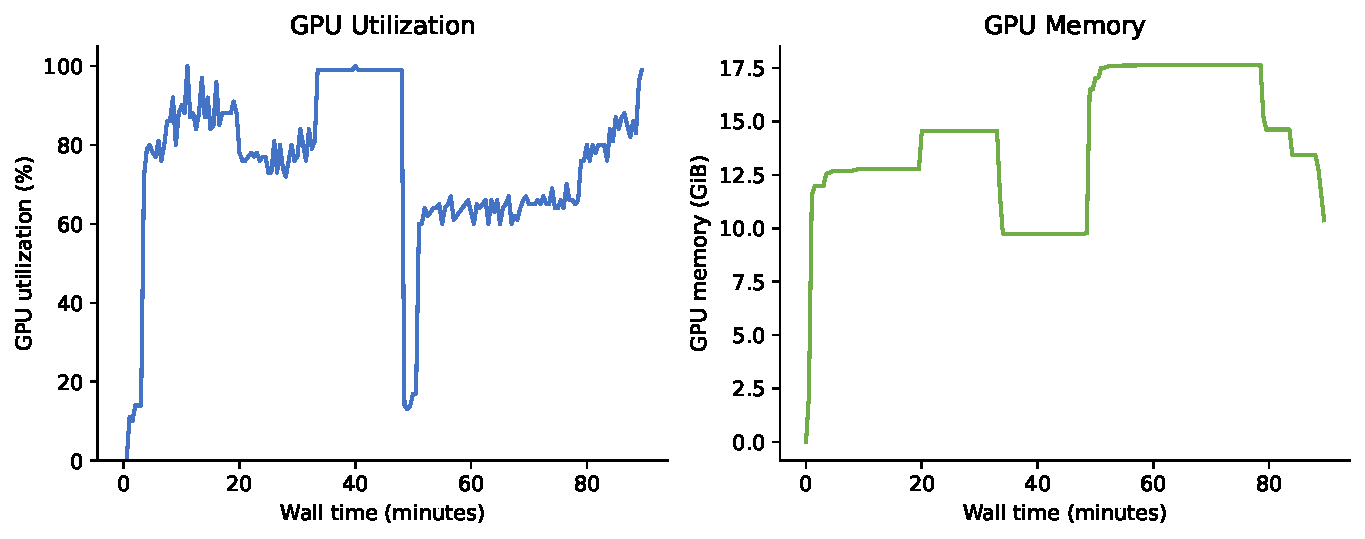
\includegraphics[width=\columnwidth]{resource_utilization}
\caption{并行任务期间的 GPU utilization 与 memory。}
\label{fig:resource}
\end{figure}

单个 actor-critic 网络计算量小，simulation 与 Python control loop 更容易成为瓶颈。
我们以独立 seed 和消融并行填充 GPU；当没有额外 scientific question 时停止扩展任务，
避免以利用率替代研究价值。

\section{局限}
第一，success 是 binary proxy，不能区分接近成功与完全失败。第二，PPO 与 off-policy
方法的 gradient update budget 不同；frames 公平比较样本效率，但不是 FLOP 公平比较。
第三，GAE 消融只有 2 seeds，主要用于诊断趋势。第四，demonstrations 来自固定 policy，
其 coverage 限制了 BC initialization。第五，Meta-World simulator 与真实机器人仍有
dynamics、latency 与 perception gap。

\section{结论}
Homework 2 展示了 RL design 的三条主线。Reward function 决定“什么是最优”；GAE 与
PPO 控制 on-policy gradient 的 bias、variance 和 update size；replay、double-Q、
ensemble 与 UTD 决定 off-policy method 如何交换 sample efficiency 与 bootstrap
stability。高质量工程实现必须把 terminal mask、target detach、target update、数据
版本与 evaluation seeds 都纳入可复现协议。

\section*{可复现性声明}
仓库提供实现、官方 demonstrations、测试、多 seed CSV、Gridworld JSON、资源记录、绘图
脚本、LaTeX 源文件与 PDF。报告数字和图片由原始指标自动生成。

\bibliographystyle{plainnat}
\bibliography{../references}
\end{document}
